\documentclass[beamer]{standalone}

%\usepackage[
%	backend=biber,
%	maxbibnames=99,
%	style=alphabetic,
%	backref=false,
%]{biblatex}
%\bibliography{../cryptobib/abbrev3,../cryptobib/crypto,../standards,../customrefs}

\usepackage{tikz}
\usetikzlibrary{positioning,decorations.pathreplacing,fit}
\usetikzlibrary{decorations.markings,shapes.arrows,arrows,arrows.meta}
\usetikzlibrary{calc}

\definecolor{mygreen}{RGB}{0,128,80}
\colorlet{darkgreen}{mygreen!90!black}


\begin{document}
\begin{standaloneframe}


\begin{tikzpicture}[
	arrow double line/.style={
		double distance = 20pt,
   		shorten <= 11, 	
   		shorten >= 16,
   		very thick,
	    postaction = {
    		draw = white,
	 	    line width = 20pt,
	 	    shorten <=-.1pt,
	 	    shorten >=-.1pt,	
	    },
	    postaction = {
	    	decorate, 
	    	decoration = {
	    		markings, 
	    		mark=at position 0 with {
	    			\arrow[xshift=26.6pt]{Straight Barb[reversed,length=-1pt 0.7]}
	    		},
	    		mark = at position 1 with {
   	    			\arrow[xshift=10.6pt]{Straight Barb[length=-1pt 0.7]}
   	    		}
	    	}
	    }
	},
	mybrace/.style= {
		decorate, decoration={brace,amplitude=5pt,raise=5pt}, thick
	},
	comment box/.style = {
		draw,inner sep = 6pt,fill=gray!25,thick,rounded corners=3pt,text=black,font=\large
	},
	every node/.style={
		font=\bfseries
	},
	]

	\def\AtB{3.7}
	\def\BtT{4.2}
	\def\InterMsgSpaceVertical{1.2}
	
	
	\node[align=center] (client) {\large C};
	\node[above=-0.2 of client] (foo) {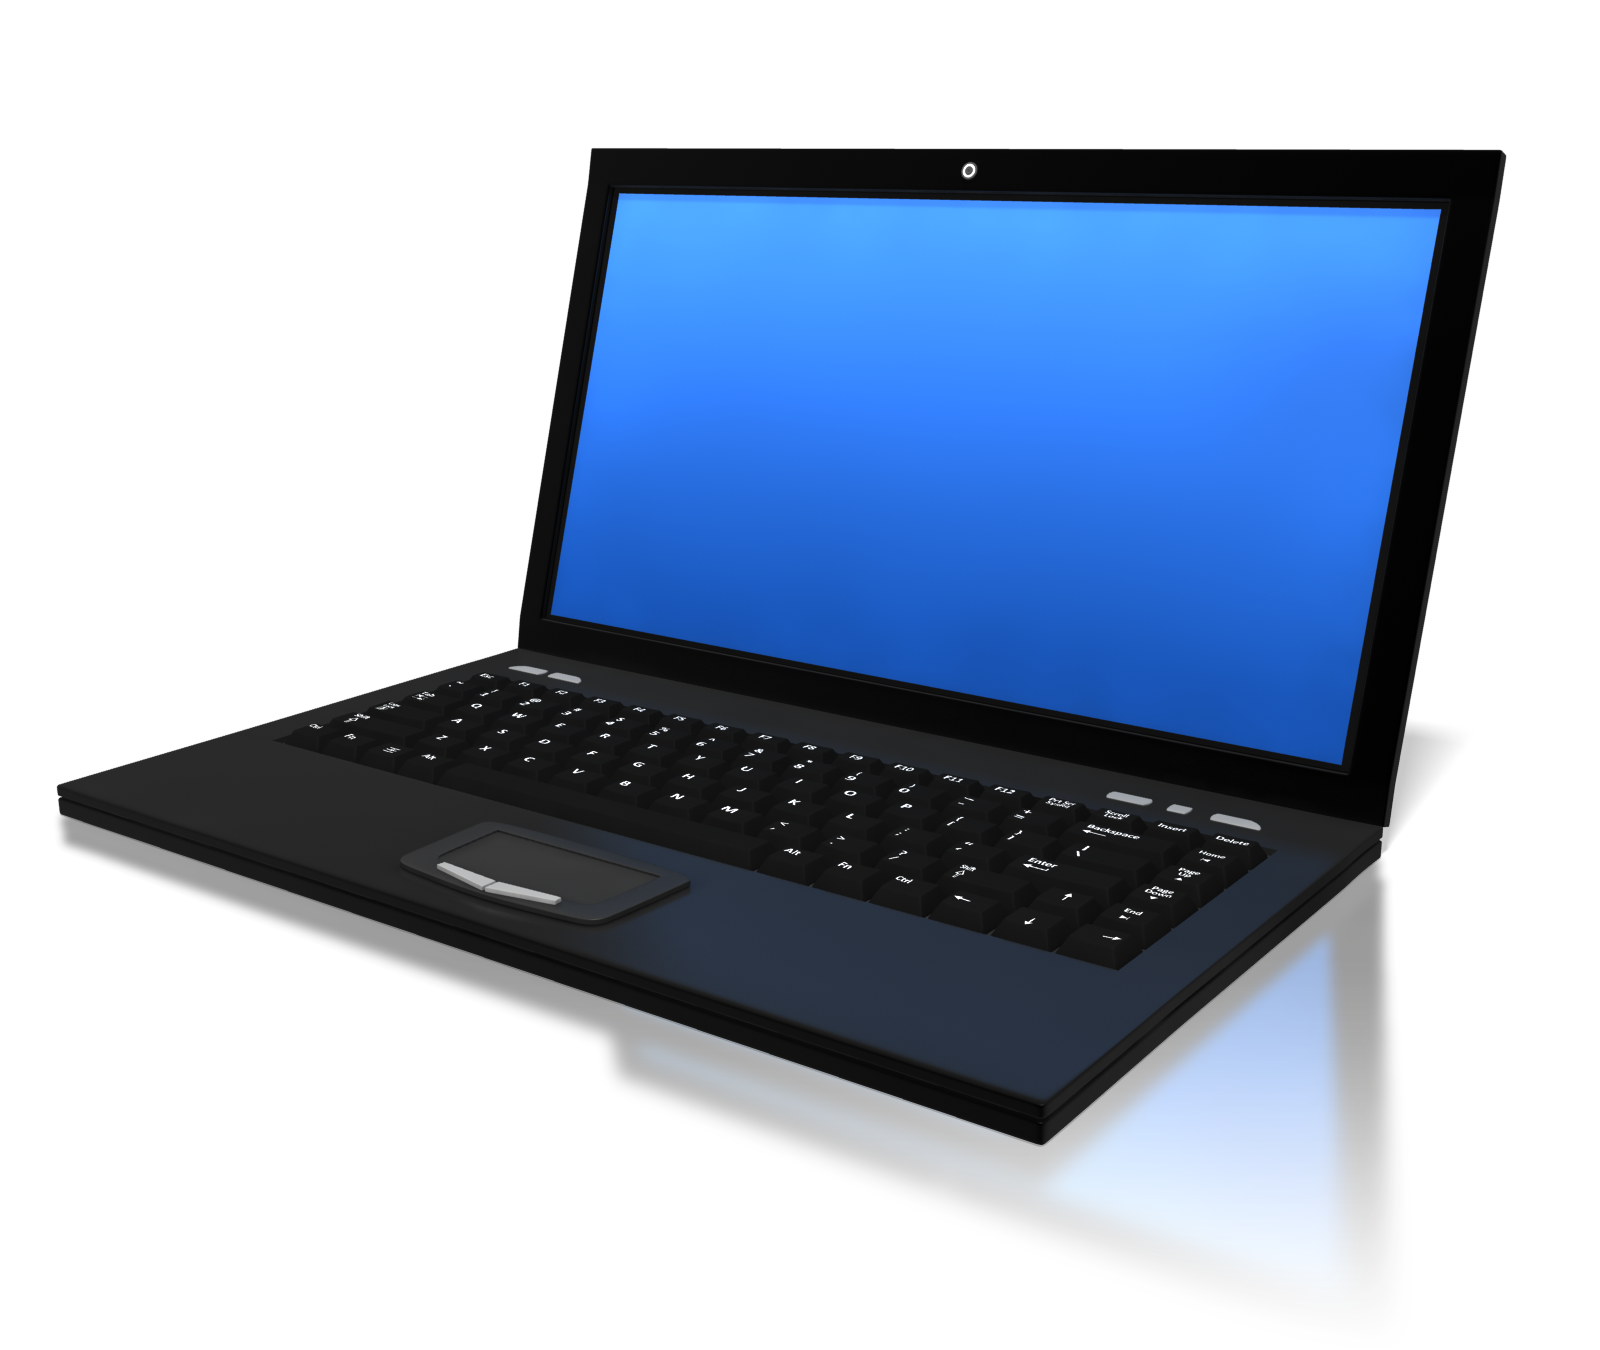
\includegraphics[width=.15\textwidth]{laptop}};
	
	\node[right = \AtB of client,align=center] (AP) {\large A};
	\node[above = 0 of AP] () {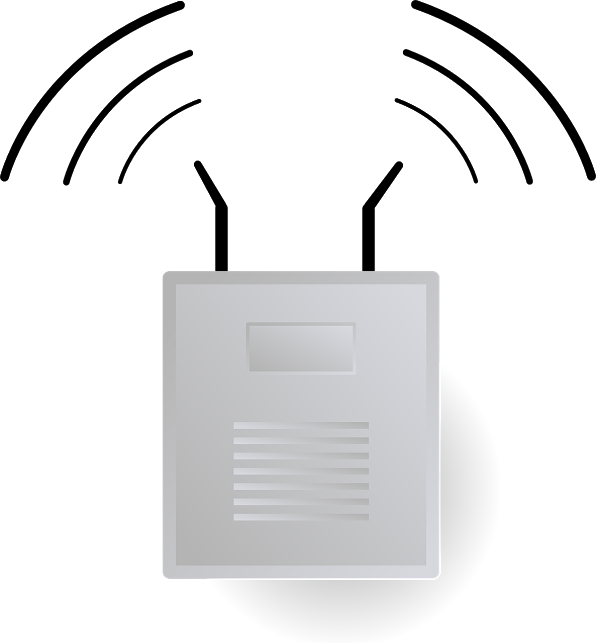
\includegraphics[width=.13\textwidth]{AP}};
	
	\node[right = \BtT of AP.east,align=center] (AS) {\large S};
	\node[above = 0 of AS] () {
\includegraphics[width=.1\textwidth]{server}};
	
	\foreach \i in {1,...,8} {
		\coordinate[below = \InterMsgSpaceVertical * (\i-1) of client] (c\i) {};
		\coordinate[below = \InterMsgSpaceVertical * (\i-1) of AP] (ap\i) {};
		\coordinate[below = \InterMsgSpaceVertical * (\i-1) of AS] (as\i) {};
	}

	\draw[arrow double line,red] (c2) -- node (EAP-TLS) {
		\alt<1->{EAP-TLS, ``C'', ``A''}{$\Pi_1$ (2P-AKE), ``C'', ``A''}
	} (as2);

	\draw[arrow double line, blue] (ap3) -- node (RADIUS) {
		\temporal<-2>{$\Pi_2$ (2P-ACCE)}{RADIUS}{RADIUS-over-TLS}
	} (as3);

	\draw[double,double distance=12, shorten >= 19, shorten <= 9, very thick, blue,
	postaction = {
	    		draw = white,
		 	    line width = 12pt,
		 	    shorten <= -.1pt,
		 	    shorten >= -.1pt,	
		    }] (as4) -- node[yshift=-13,black] {} (ap4);
	
	\draw[->,shorten >= 9.5, shorten <= 3.3,dashed,dash phase=3pt, very thick] (as4) -- (ap4);


	\node[left = 0 of c2,align=right] (p1_Ak) {
		
\includegraphics[width=.06\textwidth]{key_red} \hspace{1pt} 
		
\includegraphics[width=.06\textwidth]{key_purple}
	};


	\node[right = -0.1 of as2,align=left] (p1_Tk) {
		
\includegraphics[width=.06\textwidth]{key_red} \hspace{1pt} 
		
\includegraphics[width=.06\textwidth]{key_purple}
	};

	\node[right = -7pt of as4,align=left] (p3_Tk) {``C''\hspace{-2pt} + 
\includegraphics[width=.06\textwidth, trim=0 7cm 0 4cm]{key_purple}};	

	\node[left = -9pt of ap4,align=right] (p3_Bk) {``C''\hspace{-2pt} + 
\includegraphics[width=.06\textwidth, trim=0 7cm 0 4cm]{key_purple}};
	
	\node[draw, below left  = 1.7 and -35pt of as4, align=right,thick, inner sep=4pt] (p1_Tk) {
		$
\includegraphics[width=.06\textwidth, trim=0 7cm 0 4cm]{key_purple} 
		\gets \mathbf{KDF}(
		
\includegraphics[width=.06\textwidth, trim=0 7cm 0 4cm]{key_red},\text{``C''},\text{``A''})$
	};

	\draw[arrow double line,darkgreen] (c5) -- node[xshift=0] (4WHS) {
		\alt<1->{802.11 (4WHS)}{$\Pi_4$ (2P-AKE$^\mathsf{static}$)}
	} (ap5);
	
	\visible<5->{
		\draw[mybrace] ([xshift=1.6cm,yshift=8]as2) -- node[right=0.4,align=center] (3P-KD) {\textbf{Thm 1:}\\3P-AKE$^w$} ([xshift=1.6cm,yshift=-15]as4);
	}
	
	\visible<7->{
		\draw[mybrace, decoration={mirror}, left] ([xshift=-1.6cm,yshift=10]c2) -- node[left=0.4,align=center] {\textbf{Thm 2:}\\3P-AKE} ([xshift=-1.6cm,yshift=-15]c5);
	}
	
%	\visible<2->{
%		\node[comment box] (EAP-TLS-result) at ([xshift=10pt]c3) {\textbf{\cite{EC:BrzJacSte16}: 2P-AKE}}; 	
%		\draw[->,thick] (EAP-TLS-result) -- (EAP-TLS);
%	}
%	
%	\visible<2->{	
%		\node[comment box] (4WHS-result) at ([xshift=4cm,yshift=-1cm]ap5) {\textbf{2P-AKE$^{\mathsf{static}}$ + EA [our paper]}}; 	
%		\draw[->, thick, shorten >= -0.1cm] (4WHS-result) -- (4WHS.east);
%	}
	
	\visible<4->{
		\node[comment box] (TLS-result) at ([xshift=-3cm]AS) {\textbf{\cite[\dots]{C:JKSS12,C:KraPatWee13,PKC:LSYKS14}: 2P-ACCE}}; 	
		\draw[->,thick,shorten >= 0.2cm] (TLS-result) -- ([xshift=-0.5cm]RADIUS.east);
	}
	

	
%	\visible<6->{	
%		\node[comment box] (4WHS-result) at ([xshift=90pt,yshift=-15]ap5) {\textbf{Thm: 2P-AKE$^{\mathsf{static}}$ + EA}}; 	
%		\draw[->, thick, shorten >= -0.1cm] (4WHS-result) -- (4WHS);
%	}

\end{tikzpicture}

\end{standaloneframe}

\end{document}